\head{Ноябрь}{Листок 10. Графы. Повторение.}
\noindent
Этот листок является собранием фактов и идей, изученных в курсе 7 класса, поэтому список обязательных задач определяется для каждого в индивидуальном порядке.

\section{Простейшие определения.}

\begin{dfn}
    \textit{Графом} называется конечное множество точек на плоскости, некоторые пары которых соединены линиями. Эти точки называются \textit{вершинами} графа, а линии -- \textit{рёбрами} графа.
\end{dfn}

\begin{dfn}
    Граф, у которого каждое ребро имеет направление, называется \textit{ориентированным} \textit{графом}.
\end{dfn}

\noindent
Если каждое ребро соединяет различные вершины то мы говорим, что \textit{нет петель}, а если каждые две вершины соединены не более, чем одним ребром, то \textit{нет кратных рёбер}.

\begin{dfn}
    Количество рёбер, выходящих из данной вершины, называется степенью этой вершины. Вершина графа, имеющая нечётную степень, называется нечётной, а имеющая чётную степень -- чётной.
\end{dfn}

\begin{ex}
    Известны степени всех вершин графа. Выведите формулу для подсчёта количества ребер в этом графе.
\end{ex}

\begin{center}
  \fbox{\begin{varwidth}{0.95\textwidth}
    \begin{thrm} \label{10.3 thrm1}
        Число нечётных вершин любого графа -- чётно.
    \end{thrm}
\end{varwidth}}  
\end{center}

\begin{ex}
    Докажите теорему \ref{10.3 thrm1}.
\end{ex}

\noindent
Заметим, что теорему \ref{10.3 thrm1} часто называют леммой о рукопожатиях. Почему? Попробуйте решить такую задачу: «Докажите, что количество человек, когда либо живших на земле и сделавших за свою жизнь нечётное число
рукопожатий -– чётно». 
\\ Что общего между этой задачей и теоремой \ref{10.3 thrm1}? Чему равно количество всех рукопожатий?

\begin{ex}
    Программисты одного НИИ решили соединить имеющиеся у них 2013 компьютеров проводами так, чтобы каждый компьютер был соединен ровно с 3 другими. Удастся ли им осуществить свою идею?
\end{ex}

\begin{prf}
    Если бы это было возможно, то можно бы было нарисовать граф, где вершины являлись бы изображением компьютеров, а рёбра -– проводами. Тогда нарисованный граф имел бы 2013 нечётных вершин, что по лемме о рукопожатиях невозможно.
\end{prf}

\begin{ex}
    Рома увлекается географией и хочет нарисовать на бумаге 17 государств так, чтобы каждое из них граничило ровно с тремя другими. Сможет ли он это сделать? (Одно государство изображается одной областью на бумаге)
\end{ex}

\begin{ex}
    Докажите, что если в графе не менее двух вершин, то в нем есть вершины одинаковой степени. % (Сравните с задачей 2.20 из листка 2 «Принцип Дирихле»)
\end{ex}

\section{Формулировка условия задач в виде графа.}

\noindent
Следующие задачи ПОКА решать не нужно. Требуется ТОЛЬКО привести их переформулировку на языке графов.

\begin{ex}
    Лиза, вернувшись из осенней школы, заявила, что в школе было ровно 2013 ребят, и что в начале смены каждый из них был знаком ровно с семью другими. Права ли Лиза?
\end{ex}

\begin{ex}
    В классе 25 человек. Известно, что среди любых трёх из них есть двое друзей. Докажите, что есть ученик, у которого не менее 12 друзей.
\end{ex}

\begin{ex}
    Во дворе живут 4 пёсика: Бобик, Робик, Тобик и Толстолобик. Каждому из них случалось драться с кем-нибудь из остальных, причём у Бобика, Робика и Тобика число тех, с кем они дрались -- разное. Со сколькими собаками двора дрался Толстолобик?
\end{ex}

\begin{ex}
    Докажите, что среди девяти человек найдутся либо трое попарно знакомых, либо четверо попарно незнакомых.
\end{ex}

\begin{ex} \label{10.3 ex11}
    На плоскости нарисованы 9 точек. Максим соединил некоторые из них синим цветом, а Миша все остальные точки соединил красным. Докажите, что найдется либо синий треугольник, либо красный четырёхугольник с красными диагоналями.
\end{ex}

\begin{ex}
    В сказочной стране Перра-Терра живут карабасы и барабасы. Каждый карабас знаком с 4 барабасами и 7 карабасами, а каждый барабас знаком с 6 карабасами и 5 барабасами. Кого в стране больше – карабасов или барабасов?
\end{ex}

\begin{ex}
    Можно ли нарисовать на плоскости 9 отрезков так, чтобы каждый пересекался ровно с тремя другими?
\end{ex}

\begin{ex} \label{10.3 ex14}
    Проходит волейбольный турнир школы по круговой системе (каждая команда играет с каждой ровно один раз). Участвует 17 команд. В том числе и команда 8 класса. В некоторый момент времени оказалось, что все команды (кроме команды 8) сыграли разное количество матчей. Сколько матчей к этому моменту сыграла команда 8 класса?
\end{ex}

\begin{ex} \label{10.3 ex15}
    В кружке танцев каждая девочка познакомилась с 6 мальчиками и 7 девочками, а каждый мальчик -- с 3 девочками и 4 мальчиками. Кого в кружке больше: мальчиков или девочек?
\end{ex}

\begin{figure}[H]\begin{minipage}{0.3\linewidth}
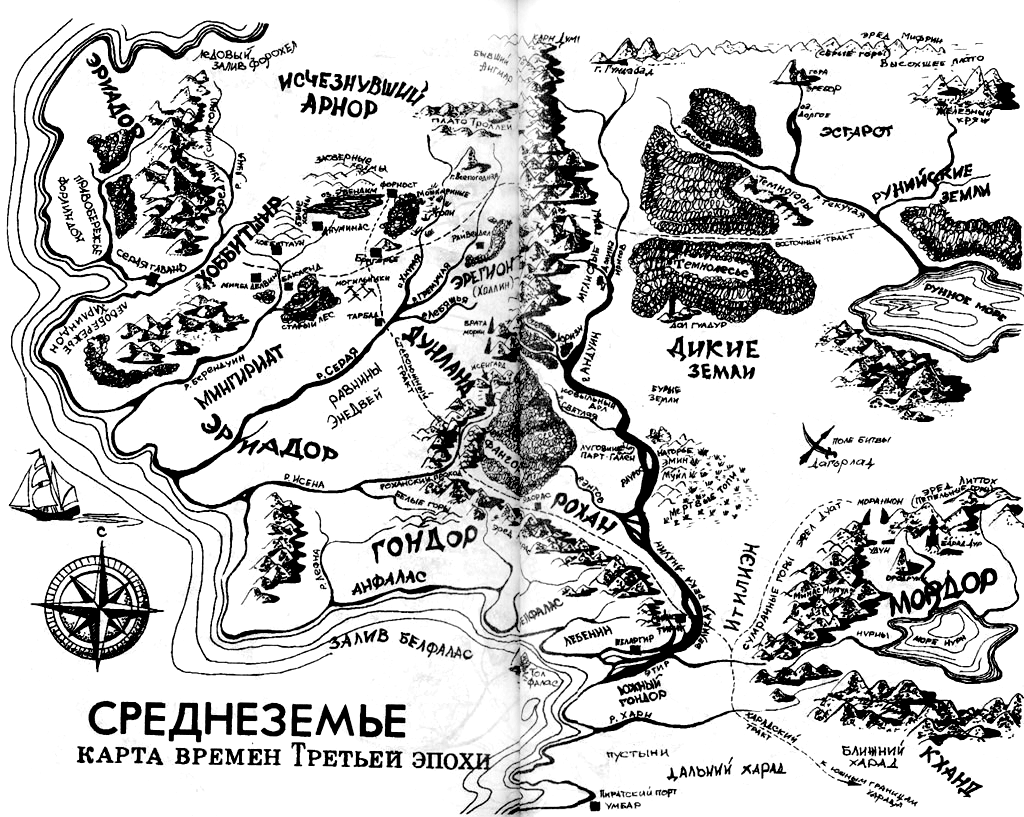
\includegraphics[width=0.95\columnwidth]{img/10.3 sredn.png}
\end{minipage}
\hfill
\begin{minipage}{0.69\linewidth}\setlength{\parindent}{1.5em}
    \begin{ex}
    Резидент одной из иностранных разведок сообщил, что пятнадцать республик бывшего Советского Союза заключили несколько двухсторонних соглашений так, что каждая из них заключила договор ровно с тремя другими. Заслуживает ли резидент доверия?
\end{ex}

\begin{ex}
    Докажите, что на любой географической карте с 2013 странами найдутся по крайней мере две страны с одинаковым числом соседей.
\end{ex}

\begin{ex} \label{10.3 ex18}
    В государстве N ровно $2n + 1$ городов. Новый президент издал указ, по которому каждый город должен быть соединен автострадой ровно с $2k + 1$ другими. Для каких значений $n$ и $k$ можно выполнить указ президента?
\end{ex}
\end{minipage}
\end{figure}

\begin{ex}
    В стране Девятка девять городов. Некоторые из них соединены авиалиниями (туда и обратно). Докажите, что либо найдутся три города, которые можно облететь по циклу, либо четыре города, ника-
кие два из которых не соединены авиалинией.
\end{ex}

\begin{ex}
    В графе каждая вершина покрашена в синий или зеленый цвет. При этом каждая синяя вершина связана с пятью синими и десятью зелеными, а каждая зеленая с девятью синими и шестью зелёными. Каких вершин больше -– синих или зелёных?
\end{ex}

\begin{ex} \label{10.3 ex21}
    У Маши 24 одноклассника, причем все они имеют различное число друзей в этом классе. Сколько из них дружат с Машей?
\end{ex}

\begin{thm}
    Докажите упражнения \ref{10.3 ex11}, \ref{10.3 ex14}, \ref{10.3 ex15}, \ref{10.3 ex18} и \ref{10.3 ex21}.
\end{thm}

\newpage

\section{Связные графы.}

\begin{ex} \label{10.3 ex22}
    В стране Семёрка 15 городов, каждый из которых соединён дорогами не менее, чем с 7 другими. Докажите, что из любого города можно добраться до любого другого (возможно, через другие города).
\end{ex}

\begin{dfn}
    Путём в графе называется последовательность ребер, каждое следующее из которых начинается в конце предыдущего, последовательность проходимых при этом вершин от А до В также называется путём, соединяющим вершины А и В.\footnotemark
\end{dfn}\footnotetext{Вообще говоря, проходимые при этом вершины и рёбра не обязаны быть различными. Путь, в котором никакие вершины и рёбра не встречаются два раза, называют простым путём. Обычно в каждом конкретном случае понятно, о каком из путей идёт речь.}

\begin{dfn}
    Замкнутый путь (т.е. путь, у которого совпадают начало и конец), не проходящий через одно ребро дважды, называется \textit{циклом}.\footnotemark
\end{dfn}\footnotetext{Т.е. цикл – это в частности простой путь. Однако цикл может иметь самопересечения, т.е. проходить дважды через одну вершину. Циклы, не проходящие дважды через одну вершину, часто также называют \textit{простыми} циклами.}

\begin{dfn}
    Связный граф, не имеющий циклов, называется \textit{деревом}.
\end{dfn}

\noindent Таким образом, решение упражнения \ref{10.3 ex22} есть доказательство того, что граф дорог страны Семёрка связен. Если граф несвязен, то в нём можно выделить \textit{компоненты связности}, т.е. «куски», являющиеся связными подграфами. Если таких кусков нельзя выделить меньше двух, то граф будет \textit{двухсвязным}, если три, то -- \textit{трёхсвязным} и т.д.

\begin{center}
  \fbox{\begin{varwidth}{0.95\textwidth}
    \begin{thrm}
        Если из каждой вершины конечного графа выходит ровно два ребра, то такой граф является либо циклическим, либо объединением циклических.
    \end{thrm}
\end{varwidth}}  
\end{center}

\begin{dfn}
    Граф называется эйлеровым, если в нём существует замкнутый путь, проходящий через все рёбра ровно по одному разу. Такой путь, соответственно, называют эйлеровым циклом.
\end{dfn}

\begin{ex}
    Приведите примеры эйлеровых графов.
\end{ex}

\begin{ques}
    Верно ли, что эйлеров цикл не имеет самопересечений, т.е. всегда является простым циклом?
\end{ques}

\begin{thm}
    В одном городе на каждом перекрёстке сходится чётное число улиц. Известно, что с любой улицы можно проехать на любую другую. Докажите (без использования критерия эйлеровости), что можно объехать все улицы города, побывав на каждой из них ровно один раз.
\end{thm}

\textit{\underline{Замечание}}: иногда в литературе эйлеровым графом называют граф, в котором существует путь (т.е. не обязательно замкнутый), проходящий через все рёбра ровно по одному разу. Будем называть такой граф \textit{почти эйлеровым}. В частности любой эйлеров граф является почти эйлеровым, т.к. любой цикл является путём. Примером почти эйлеровых графов являются фигуры, которые можно нарисовать, не отрывая карандаша от бумаги и не проводя ни по каким линиям дважды.

\begin{center}
  \fbox{\begin{varwidth}{0.95\textwidth}
    \begin{thrm} 
        \textit{(необходимое условие почти эйлеровости графа)} Если граф является почти эйлеровым, то он имеет не более одной компоненты связности с ненулевым количеством рёбер и не более двух нечётных вершин. Это же условие является и достаточным для связных графов.
    \end{thrm}
    \begin{thrm}
        \textit{(критерий эйлеровости связного графа)} Граф является эйлеровым тогда и только тогда, когда каждая его вершина имеет чётную степень. (Эта теорема обсуждалась в прошлом году)
    \end{thrm}
\end{varwidth}}  
\end{center}

\textbf{Вопрос.} Является ли полный граф с 10-ю вершинами эйлеровым?

\begin{thm}
    В стране Миллениум некоторые города связаны между собой авиалиниями. Из столицы выходит 2013 авиалиний, из города Тьма-Таракань -- одна, а из всех остальных городов -- ровно по 2012 авиалинии. Можно ли из Тьмы-Таракани добраться в столицу?
\end{thm}

\begin{thm}
    Может ли в государстве, в котором из каждого города выходит 3 дороги, быть ровно 100 дорог?
\end{thm}



\begin{figure}[H]
\begin{minipage}{0.69\linewidth}\setlength{\parindent}{1.5em}
    \begin{thm}
    В стране Стодорожной из каждого города выходит ровно 100 дорог и из любого города можно проехать в любой другой. Одну из дорог закрыли на ремонт. Докажите, что и теперь можно добраться из любого города в любой другой.
    \end{thm}
    \begin{thm}
        На рисунке изображён план первого этажа дома. Можно ли составить маршрут обхода этого этажа так, чтобы он проходил через каждую дверь ровно один раз?
    \end{thm}
\end{minipage}
\hfill
\begin{minipage}{0.3\linewidth}
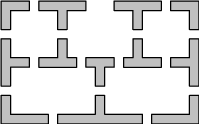
\includegraphics[width=0.95\columnwidth]{img/10.3 staircase.png}
\end{minipage}
\end{figure}

\begin{thm}
    Назовём граф «хлипким», если степень любой его вершины равна 1, 3 или 6. Докажите, что из связного «хлипкого» графа, содержащего 34 ребра, можно выкинуть ребро так, что он перестанет быть связным.
\end{thm}

\begin{thm}
    Каждый из 17 учёных переписывается с остальными. В их переписке речь идёт о трёх темах. Каждая пара учёных переписывается друг с другом лишь по одной теме. Доказать, что не менее трёх учёных переписываются друг с другом по одной теме.
\end{thm}

\begin{thm}
    Верно ли что во всяком графе с 16 вершинами и степенью 3 у каждой вершины можно выбрать 8 рёбер так, чтобы на них лежали все вершины?
\end{thm}